% !TeX spellcheck = de_DE

\chapter{Verfügbare Technologien}
\label{chap:sota}

Im Kapitel wird auf verschiedene Arbeiten zum Thema autonome Flugplanung und Hinderniserkennung eingegangen. Zuerst werden die beiden Arbeiten des vorhergehenden Jahrgangs betrachtet. Weiterhin wurden bereits Forschungen zum Thema durchgeführt, welche als Ausgangspunkt für diese Arbeit genutzt werden. Außerdem werden Algorithmen zur kamerabasierten Bilderkennung eingeführt, da derartige von verkaufsfertigen Produkten verwendet werden. %verfügbare Technologien für den autonomen Drohnenflug vorgestellt und ausgewertet. Dabei wird auf verfügbare Hard- und Software Lösungen eingegangen.

\section{Vorraussetzungen aus dem ersten Projektteil}
Im ersten Projektteil, siehe \cite{wirthErweiterungBestehendenDrohne2022}, wurden die Grundlagen zum autonomen Drohnenflug erarbeitet. Es wurde der Markt an verfügbaren Drohnen analysiert, um die best-geeignetste Drohne herauszusuchen\cite[Kapitel 3]{wirthErweiterungBestehendenDrohne2022}. Zur Entwicklung ausgewählt wurde das Modell \enquote{Holybro S500}\cite[Kapitel 4.3]{wirthErweiterungBestehendenDrohne2022}, welches in dieser Arbeit weiterhin verwendet wird. Der Quadcopter hat folgende Eigenschaften:
\begin{compactitem}
	\item Gewicht: 935g, Gesamtgewicht mit Akku, Sensoren und Bordcomputer: ?
	\item Traglast: 1,8kg
	\item Akku: Typ - LiPo; Nennspannung - 14,8V; Kapazität - 5000mAh; Capacity-Racting: 10C; Gewicht - ?
	\item Flugcontroller: \gls{px4}
	\item Sensoren: Gyroskop, Beschleunigung, Kompass, Barometer, \acrshort{gps}
\end{compactitem}

Um den autonomen Flug planen zu können, wären mögliche Fluggeschwindigkeit und Flugdauer notwendig. Dazu ist keine Angabe vom vorhergehenden Projekt bekannt, die Werte werden in diesem Projekt ermittelt.

Der gesamte Aufbau des Systems ist in Abbildung \ref{fig:systemaufbau} gezeigt. Die Modelldrohne und ihre zusätzliche Peripherie gliedert sich folgendermaßen:
\begin{compactdesc}
    \item[Flugcontroller:] Kontrolle der originalen Drohne
    \item[\gls{rpi}:] Bordcomputer, kommuniziert direkt mit dem Flugcontroller und den Ultraschallsensoren; stellt WLAN-Netzwerk bereit
	\item[\gls{gcs}\footnote{Bodenstation}:] Laptop/Smartphone der Flug steuert und Drohne parametriert; zum Einsatz kommt die Software QGroundControl, siehe \cite[Kapitel 4.3.5]{wirthErweiterungBestehendenDrohne2022}
    \item[Ultraschallsensoren:] 4 Stück; Erfassen von Hindernissen in der Umgebung; ausgerichtet nach vorn/oben/unten
    \item[Kamera:] verbunden mit \gls{rpi}; nicht für dieses Projekt bereitgestellt
\end{compactdesc}

\begin{figure}[!h]
	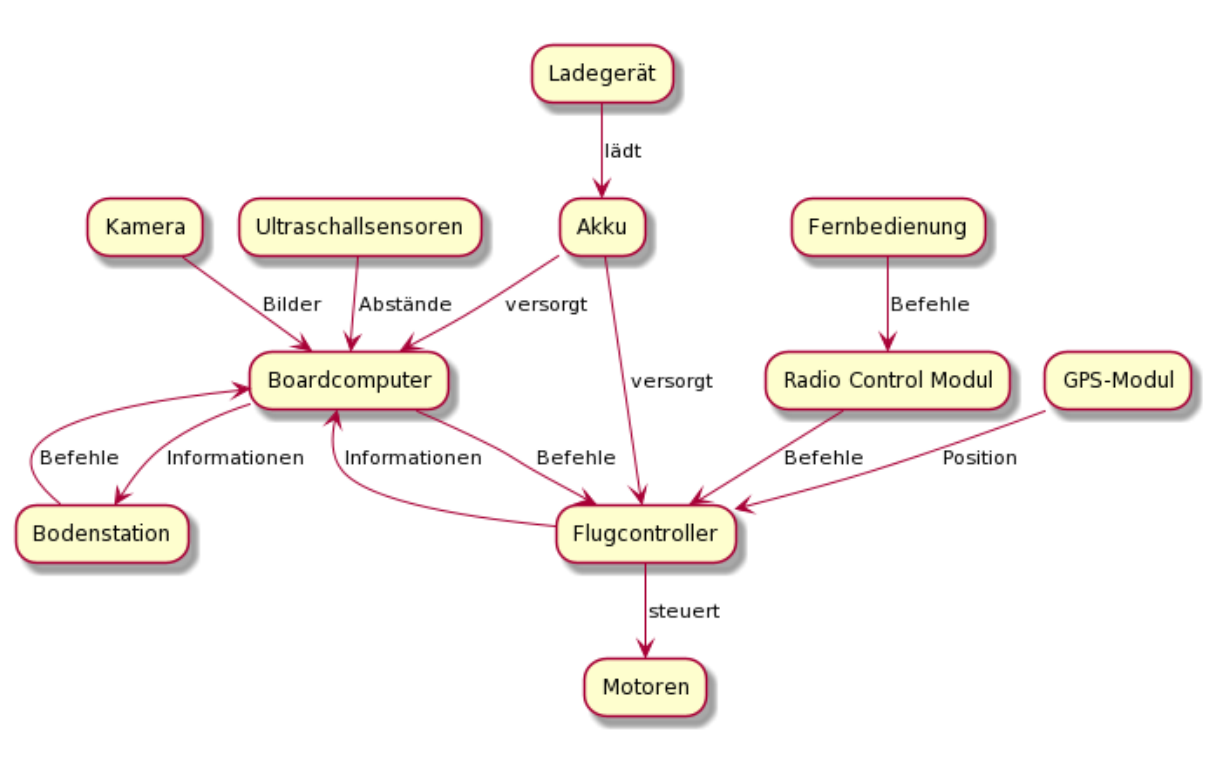
\includegraphics[width=\linewidth]{images/systemuebersicht.png}
	\caption{Systemübersicht mit allen physischen Bauteilen\cite[Kapitel 4.3]{wirthErweiterungBestehendenDrohne2022}}
	\label{fig:setup_initial}
	\end{figure}

Mit den Sensoren können Objekte in der Flugbahn detektiert werden, solange die Bewegung entlang einer der Raumrichtungen: \enquote{Oben},\enquote{Unten} oder \enquote{Vorwärts} stattfindet. Zusammengesetzte Bewegungen dürften nicht durchgeführt werden, auch darf sich die Drohne nicht seitwärts oder rückwärts bewegen.

Für die Wahl der Sensoren standen ökonimische und technische Gründe im Vordergrund: anderweitige Sensoren sind entweder teuer oder verbrauchen sehr viel Strom, was die Flugdauer der Drohne drastisch senken würde\cite[Kapitel 4.3.8]{wirthErweiterungBestehendenDrohne2022}.

Die Drohne wurde mithilfe der Software QGroundControl eingerichtet\cite[Kapitel 4.3.5]{wirthErweiterungBestehendenDrohne2022} und auf Flugfähigkeit getestet\cite[Kapitel 4.3.7]{wirthErweiterungBestehendenDrohne2022}. Zum Einsatz kam eine RC-Fernsteuerung, welche nicht diesem Projekt nicht zur Verfügung steht. Als Alternative Steuerung kann entweder nur per \gls{gps} Navigation geflogen werden, oder ein virtueller Joystick von QGroundControl verwendet werden.

\section{Vorraussetzungen aus dem zweiten Projektteil}
Im zweiten Projektteil \cite{wirthErweiterungBestehendenDrohne2022a} die Software zum autonomen Flug eingeführt. Dabei traten folgende Probleme auf: das \enquote*{Meta-Betriebssystem} \gls{ros}, eingesetzt zum Auslesen der Ultraschallsensoren und Steuerung des Flugcontroller, ließ sich nicht auf dem \gls{rpi} installieren. Es wurde die Software \enquote{Docker} eingeführt, um \gls{ros} per Virtualisierung nutzen zu können\cite[Kapitel 6.5]{wirthErweiterungBestehendenDrohne2022a}.

Außerdem wurde die Kamera\cite[Kapitel 6.8]{wirthErweiterungBestehendenDrohne2022a} ausgelesen, die Ultraschallsensoren getestet\cite[Kapitel 6.9]{wirthErweiterungBestehendenDrohne2022a}, und die Navigation mittels \gls{gps} verfiziert\cite[Kapitel 6.10]{wirthErweiterungBestehendenDrohne2022a}.

Mit dem bestehenden System wurden Flugtests durchgeführt. Alle Tests wurden, mit einer Ausnahme, erfolgreich abgeschlossen. Kaum möglich ist das erkennen nicht-flächiger Hindernisse mit Ultraschallsensoren\cite[Kapitel 6.10]{wirthErweiterungBestehendenDrohne2022a}. Die gesamte bereitgestellte Software wird in Kapitel \cref{chap:einarbeite} nachvollzogen, überprüft, verbessert und angepasst.

Als Bestandteil der Arbeit wurde ein Simulator, um \enquote{ein[en] Algorithmus zur Hindernisumgehung, der auf die reale Hardware übertragen werden soll [zu entwickeln]. Dieser Algorithmus soll in der Simulation implementiert und getestet werden.}\cite[Kapitel 8]{wirthErweiterungBestehendenDrohne2022a}. Somit wird die Entwicklung und das Testen der Funktionalität vereint und kann fließend erfolgen. Der Ansatz wird für diese Arbeit übernommen. 


\section{Marktreife Anwendungen}
Der Drohnenmarkt gehört so gut wie der Firma \enquote{DJI} allein, nach \cite{StatistikDrohnenVerkaeufeNach}. Die Drohnen der Firma verwenden zur Hinderniserkennung verschiedene SLAM-Algorithmen\cite{ciobanuObstacleAvoidanceDJI2021}, siehe \cref{chap:slam}. Dabei kommen immer mehrere Sensoren zum Einsatz deren Messdaten überlagert werden. Nach \cite{ciobanuObstacleAvoidanceDJI2021} werden folgende Sensoren verwendet:
\begin{compactdesc}
    \item[Ultraschall Sensor:] Beschrieben in \cref{chap:ultrasonic}
    \item[Infrarot Sensor:] Sendet Infrarot-Signale aus und misst anhand von Stärke von Reflektionen die Entfernung zu Objekten; funktioniert nicht bei Sonnenlicht
    \item[Time of Flight Sensor:] Beleuchtung einer Szene und Messung der Laufzeit der Lichtwellen; erfasst gesamtes Bild
    \item[LIDAR:] Beleuchtung eines Punktes und Messung der Laufzeit der Lichtwellen; erfasst einen Punkt
    \item[Stereokamera:] Verwendung mehrerer Kameras zur Erkennung und Messung von Objekten in Bildern; beschrieben in \cref{chap:stereovision} 
\end{compactdesc} 

Kameras befinden sich zumeist nur nach vorn (oder unten) gerichtet, arbeiten also in Flugrichtung. Ultraschall- und Infrarot Sensoren werden rundherum eingesetzt um Abstände zu weiteren Objekten abzuschätzen. Andere Sensoren kommen laut \cite{ciobanuObstacleAvoidanceDJI2021} nicht zum Einsatz (oder sind aus Konkurrenzzwecken nicht dokumentiert). 

Außerdem bei Hobby-Anwendern im Internet weit verbreitet\footnote{Bspw. \url{https://www.youtube.com/watch?v=p8frNNYQNV4}, \url{https://www.youtube.com/watch?v=f0HoyJbYCPQ}}, sind Projekte basierend auf \enquote{Intel RealSense}-Produkten. Derartige Kameras stellen ein hochauflösendes Bild mit Tiefeninformationen zur Verfügung. Dazu werden Stereo- und Infrarot Kameras und ausgeklügelte Algorithmen verwendet. Jedoch sind dem Autor keine Erfolge im für diese Projekt geforderten Umfang bekannt.

Alle Anwendungen außer einfachen Ultraschallsensoren und Kameras sind nach \cite[Kapitel 4.3.8]{wirthErweiterungBestehendenDrohne2022} nicht für dieses Projekt geeignet und werden nicht weiter in Betracht gezogen.

\section{Pixhawk Software}
Die Software des Flugcontrollers \enquote{Pixhawk}, Ursprünglich entwickelt von Lorenz Meier et al., bietet umfangreiche Anleitungen zur Entwicklung neuer Software. Diese werden im Projekt aufgegriffen und verwendet.
\subsection{Simulator}
In \cite[Kapitel 6.5]{wirthErweiterungBestehendenDrohne2022a} wurde erarbeite, dass die Simulationssoftware \enquote{Gym Pybullet Drone}\footnote{\url{https://github.com/utiasDSL/gym-pybullet-drones}\cite{paneratiLearningFlyGym2021}} am einfachsten zu bedienen sei. In den Anleitungen des Pixhawk\footnote{\url{https://docs.px4.io/main/en/simulation/}}\cite{dronecodestiftungPX4UserGuide} ist diese allerdings nicht aufgeführt. Stattdessen empfohlen wird die Software \enquote{Gazebo}. Mit ihr können beliebige Drohnen in beliebigen Umgebungen simuliert werden und auch die Integration von \gls{ros} ist vorgesehen. Eine solche Konfiguration ist vereinfacht dargestellt in Bild \ref{fig:sim1}. Allerdings wird angenommen, dass \gls{ros} direkt auf dem Flugcontroller zusammen mit der PX4-Software ausgeführt wird. Die realen Bedingungen hingegen entsprechen dem Aufbau in Bild \ref{fig:sim2}. Da es nicht notwendig sein sollte, die Software des Flugcontrollers zu verändern, ist es auch nicht notwendig offiziell unterstützte Software zu verwenden. Weiterhin muss die Entwicklung auf einem Windows® PC stattfinden. \textit{Gym Pybullet Drone} vergleicht sich selbst mit Alternativen, unter anderem \enquote{AirSim}\footnote{\url{https://github.com/microsoft/AirSim}\cite{WelcomeAirSim2023}} von Microsoft. Dieses wird auch von \textit{Pixhawk} unterstützt und steht als ausführbare Datei bereit. Auch kann der Flugcontroller direkt mit \textit{AirSim} verbunden werden, sodass ein \gls{hil} Aufbau wie in Bild \ref{fig:sim3} bereit steht. Nachteilig ist, dass das Programm eingestellt werden soll. Aufgrund der umfangreichen Anleitungen zur Einrichtung bereit\cite[siehe \enquote*{documentation}]{WelcomeAirSim2023} soll es trotzdem während dieses Projektes zur Entwicklung verwedet werden.

\begin{figure}
    \centering
    \begin{subfigure}{0.3\linewidth}
        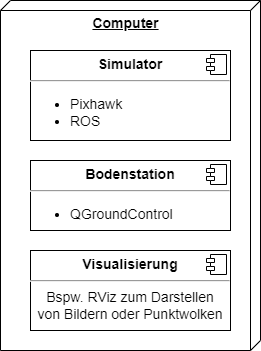
\includegraphics[width=\linewidth]{images/setup_simulator-Page-1.drawio.png}
        \caption{Offizieller Simulator vereint Flugcontroller und \acrshort{ros}}
        \label{fig:sim1}
        \end{subfigure}
    \hfill
    \begin{subfigure}{0.5\linewidth}
        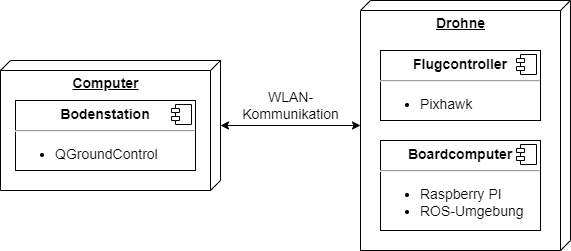
\includegraphics[width=\linewidth]{images/setup_simulator-Page-2.drawio.png}
        \caption{Gegebener Aufbau aus Hardware}
        \label{fig:sim2}
        \end{subfigure}
    \hfill
    \begin{subfigure}{0.7\linewidth}
        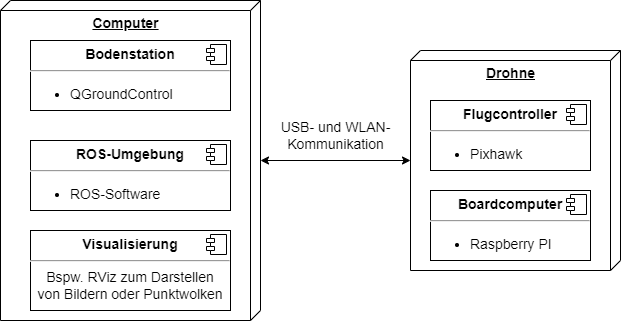
\includegraphics[width=\linewidth]{images/setup_simulator-Page-3.drawio.png}
        \caption{Gegebener Aufbau mit \textit{AirSim}}
        \label{fig:sim3}
        \end{subfigure}
         
    \caption{Systemübersicht in Hardware und im Simulator}
    \label{fig:simulator_aufbauten}
    \end{figure}

\subsection{PX4 \enquote{Obstacle Detection and Avoidance}}
Weitere Arbeiten bezüglich des Autonomen Fluges auf die dieses Projekt aufbauen kann, wurden von Lorenz Meier in Auftrag gegeben. Als Resultat entstanden, unter anderem zwei Master-Arbeiten und, das Verzeichnis\footnote{\url{https://github.com/PX4/PX4-Avoidance}\cite{dronecodestiftungPX4UserGuide}}. Dort sind Algorithmen zur Hinderniserkennung, Wegplanung und Navigation analysiert und notwendige \acrshort{ros}-Knotenpunkte bereits definiert. Sie müssen nur noch eingebunden werden.

Zur Implementation kamen bisher nur \textit{Intel RealSense} Kameras in Verbindung mit leistungsstarker Hardware (bspw. PC, Nvidia Jetson) zum Einsatz. Die \acrshort{ros}-Knotenpunkte benötigen eine Tiefenkarte, welche direkt von der Kamera bereitgestellt wird. Ein anderer Anwendungsfall ist nicht beschrieben.

Somit besteht die Aufgabe dieses Projektes darin, entsprechende Tiefenkarte zu generieren, dem Wegplanungsalgorithmus zuzuführen und schließlich dem Flugcontroller das Ergebnis einzuspielen.

%\subsubsection{A*-Algorithmus}
%Der am weitesten verbreitete Algorithmus zur Wegsuche ist der A*-Algorithmus. Er sucht den kürzesten Weg in einem Graph basierend auf Kantengewichten zwischen Knoten.
%Bei der Anwendung in Computerspielen wird die Karte dazu als Raster aus Knoten dargestellt. Je nach Weglänge ergibt sich ein Kantengewicht für die Verbindung zweier Knoten.
%Die Schwierigkeit bei der Anwendung von A* in realen Systemen ist es, kontinuierliche Umgebungsinformationen auf einem Raster darzustellen. Je höher die Anzahl an Punkten im Raster, umso exponentiell höher ist der benötigte Rechenaufwand. Bei wenigen Punkten sinkt jedoch die Auflösung, was zu groben Fehlern der Flugplanung führen kann.
%
%\subsubsection{D*-Algortihmus}
%\subsubsection{Obstacle Tracing}
%\subsubsection{Dynamic Pathfinding Algorithm}
%\subsubsection{Rapidly-exploring random trees (RRT)}
%
%
